\documentclass[]{article}
\usepackage{lmodern}
\usepackage{amssymb,amsmath}
\usepackage{ifxetex,ifluatex}
\usepackage{fixltx2e} % provides \textsubscript
\ifnum 0\ifxetex 1\fi\ifluatex 1\fi=0 % if pdftex
  \usepackage[T1]{fontenc}
  \usepackage[utf8]{inputenc}
\else % if luatex or xelatex
  \ifxetex
    \usepackage{mathspec}
  \else
    \usepackage{fontspec}
  \fi
  \defaultfontfeatures{Ligatures=TeX,Scale=MatchLowercase}
\fi
% use upquote if available, for straight quotes in verbatim environments
\IfFileExists{upquote.sty}{\usepackage{upquote}}{}
% use microtype if available
\IfFileExists{microtype.sty}{%
\usepackage{microtype}
\UseMicrotypeSet[protrusion]{basicmath} % disable protrusion for tt fonts
}{}
\usepackage[margin=1in]{geometry}
\usepackage{hyperref}
\hypersetup{unicode=true,
            pdftitle={Project\_583\_Canada},
            pdfauthor={Sofia Bahmutsky},
            pdfborder={0 0 0},
            breaklinks=true}
\urlstyle{same}  % don't use monospace font for urls
\usepackage{color}
\usepackage{fancyvrb}
\newcommand{\VerbBar}{|}
\newcommand{\VERB}{\Verb[commandchars=\\\{\}]}
\DefineVerbatimEnvironment{Highlighting}{Verbatim}{commandchars=\\\{\}}
% Add ',fontsize=\small' for more characters per line
\usepackage{framed}
\definecolor{shadecolor}{RGB}{248,248,248}
\newenvironment{Shaded}{\begin{snugshade}}{\end{snugshade}}
\newcommand{\AlertTok}[1]{\textcolor[rgb]{0.94,0.16,0.16}{#1}}
\newcommand{\AnnotationTok}[1]{\textcolor[rgb]{0.56,0.35,0.01}{\textbf{\textit{#1}}}}
\newcommand{\AttributeTok}[1]{\textcolor[rgb]{0.77,0.63,0.00}{#1}}
\newcommand{\BaseNTok}[1]{\textcolor[rgb]{0.00,0.00,0.81}{#1}}
\newcommand{\BuiltInTok}[1]{#1}
\newcommand{\CharTok}[1]{\textcolor[rgb]{0.31,0.60,0.02}{#1}}
\newcommand{\CommentTok}[1]{\textcolor[rgb]{0.56,0.35,0.01}{\textit{#1}}}
\newcommand{\CommentVarTok}[1]{\textcolor[rgb]{0.56,0.35,0.01}{\textbf{\textit{#1}}}}
\newcommand{\ConstantTok}[1]{\textcolor[rgb]{0.00,0.00,0.00}{#1}}
\newcommand{\ControlFlowTok}[1]{\textcolor[rgb]{0.13,0.29,0.53}{\textbf{#1}}}
\newcommand{\DataTypeTok}[1]{\textcolor[rgb]{0.13,0.29,0.53}{#1}}
\newcommand{\DecValTok}[1]{\textcolor[rgb]{0.00,0.00,0.81}{#1}}
\newcommand{\DocumentationTok}[1]{\textcolor[rgb]{0.56,0.35,0.01}{\textbf{\textit{#1}}}}
\newcommand{\ErrorTok}[1]{\textcolor[rgb]{0.64,0.00,0.00}{\textbf{#1}}}
\newcommand{\ExtensionTok}[1]{#1}
\newcommand{\FloatTok}[1]{\textcolor[rgb]{0.00,0.00,0.81}{#1}}
\newcommand{\FunctionTok}[1]{\textcolor[rgb]{0.00,0.00,0.00}{#1}}
\newcommand{\ImportTok}[1]{#1}
\newcommand{\InformationTok}[1]{\textcolor[rgb]{0.56,0.35,0.01}{\textbf{\textit{#1}}}}
\newcommand{\KeywordTok}[1]{\textcolor[rgb]{0.13,0.29,0.53}{\textbf{#1}}}
\newcommand{\NormalTok}[1]{#1}
\newcommand{\OperatorTok}[1]{\textcolor[rgb]{0.81,0.36,0.00}{\textbf{#1}}}
\newcommand{\OtherTok}[1]{\textcolor[rgb]{0.56,0.35,0.01}{#1}}
\newcommand{\PreprocessorTok}[1]{\textcolor[rgb]{0.56,0.35,0.01}{\textit{#1}}}
\newcommand{\RegionMarkerTok}[1]{#1}
\newcommand{\SpecialCharTok}[1]{\textcolor[rgb]{0.00,0.00,0.00}{#1}}
\newcommand{\SpecialStringTok}[1]{\textcolor[rgb]{0.31,0.60,0.02}{#1}}
\newcommand{\StringTok}[1]{\textcolor[rgb]{0.31,0.60,0.02}{#1}}
\newcommand{\VariableTok}[1]{\textcolor[rgb]{0.00,0.00,0.00}{#1}}
\newcommand{\VerbatimStringTok}[1]{\textcolor[rgb]{0.31,0.60,0.02}{#1}}
\newcommand{\WarningTok}[1]{\textcolor[rgb]{0.56,0.35,0.01}{\textbf{\textit{#1}}}}
\usepackage{graphicx,grffile}
\makeatletter
\def\maxwidth{\ifdim\Gin@nat@width>\linewidth\linewidth\else\Gin@nat@width\fi}
\def\maxheight{\ifdim\Gin@nat@height>\textheight\textheight\else\Gin@nat@height\fi}
\makeatother
% Scale images if necessary, so that they will not overflow the page
% margins by default, and it is still possible to overwrite the defaults
% using explicit options in \includegraphics[width, height, ...]{}
\setkeys{Gin}{width=\maxwidth,height=\maxheight,keepaspectratio}
\IfFileExists{parskip.sty}{%
\usepackage{parskip}
}{% else
\setlength{\parindent}{0pt}
\setlength{\parskip}{6pt plus 2pt minus 1pt}
}
\setlength{\emergencystretch}{3em}  % prevent overfull lines
\providecommand{\tightlist}{%
  \setlength{\itemsep}{0pt}\setlength{\parskip}{0pt}}
\setcounter{secnumdepth}{0}
% Redefines (sub)paragraphs to behave more like sections
\ifx\paragraph\undefined\else
\let\oldparagraph\paragraph
\renewcommand{\paragraph}[1]{\oldparagraph{#1}\mbox{}}
\fi
\ifx\subparagraph\undefined\else
\let\oldsubparagraph\subparagraph
\renewcommand{\subparagraph}[1]{\oldsubparagraph{#1}\mbox{}}
\fi

%%% Use protect on footnotes to avoid problems with footnotes in titles
\let\rmarkdownfootnote\footnote%
\def\footnote{\protect\rmarkdownfootnote}

%%% Change title format to be more compact
\usepackage{titling}

% Create subtitle command for use in maketitle
\providecommand{\subtitle}[1]{
  \posttitle{
    \begin{center}\large#1\end{center}
    }
}

\setlength{\droptitle}{-2em}

  \title{Project\_583\_Canada}
    \pretitle{\vspace{\droptitle}\centering\huge}
  \posttitle{\par}
    \author{Sofia Bahmutsky}
    \preauthor{\centering\large\emph}
  \postauthor{\par}
      \predate{\centering\large\emph}
  \postdate{\par}
    \date{16/04/2020}


\begin{document}
\maketitle

\hypertarget{section}{%
\paragraph{1.}\label{section}}

Loading the Canada data, goes up to April 24

\begin{Shaded}
\begin{Highlighting}[]
\KeywordTok{library}\NormalTok{(ggplot2)}
\KeywordTok{library}\NormalTok{(dplyr)}
\end{Highlighting}
\end{Shaded}

\begin{verbatim}
## 
## Attaching package: 'dplyr'
\end{verbatim}

\begin{verbatim}
## The following objects are masked from 'package:stats':
## 
##     filter, lag
\end{verbatim}

\begin{verbatim}
## The following objects are masked from 'package:base':
## 
##     intersect, setdiff, setequal, union
\end{verbatim}

\begin{Shaded}
\begin{Highlighting}[]
\KeywordTok{library}\NormalTok{(timelineR)}
\KeywordTok{library}\NormalTok{(data.table)}
\end{Highlighting}
\end{Shaded}

\begin{verbatim}
## 
## Attaching package: 'data.table'
\end{verbatim}

\begin{verbatim}
## The following objects are masked from 'package:dplyr':
## 
##     between, first, last
\end{verbatim}

\begin{Shaded}
\begin{Highlighting}[]
\KeywordTok{library}\NormalTok{(forecast)}
\end{Highlighting}
\end{Shaded}

\begin{verbatim}
## Registered S3 method overwritten by 'quantmod':
##   method            from
##   as.zoo.data.frame zoo
\end{verbatim}

\begin{Shaded}
\begin{Highlighting}[]
\KeywordTok{library}\NormalTok{(tidyr)}
\KeywordTok{library}\NormalTok{(gdata)}
\end{Highlighting}
\end{Shaded}

\begin{verbatim}
## gdata: read.xls support for 'XLS' (Excel 97-2004) files ENABLED.
\end{verbatim}

\begin{verbatim}
## 
\end{verbatim}

\begin{verbatim}
## gdata: read.xls support for 'XLSX' (Excel 2007+) files ENABLED.
\end{verbatim}

\begin{verbatim}
## 
## Attaching package: 'gdata'
\end{verbatim}

\begin{verbatim}
## The following objects are masked from 'package:data.table':
## 
##     first, last
\end{verbatim}

\begin{verbatim}
## The following objects are masked from 'package:dplyr':
## 
##     combine, first, last
\end{verbatim}

\begin{verbatim}
## The following object is masked from 'package:stats':
## 
##     nobs
\end{verbatim}

\begin{verbatim}
## The following object is masked from 'package:utils':
## 
##     object.size
\end{verbatim}

\begin{verbatim}
## The following object is masked from 'package:base':
## 
##     startsWith
\end{verbatim}

\begin{Shaded}
\begin{Highlighting}[]
\KeywordTok{library}\NormalTok{(stringr)}
\end{Highlighting}
\end{Shaded}

\begin{Shaded}
\begin{Highlighting}[]
\CommentTok{\#\#\# second data set}
\NormalTok{cases\_}\DecValTok{2}\NormalTok{ \textless{}{-}}\StringTok{ }\KeywordTok{read.csv}\NormalTok{(}\StringTok{"/Users/Sofia/Desktop/Data583Project/canada{-}covid19/cases\_2.csv"}\NormalTok{, }\DataTypeTok{stringsAsFactors =}\NormalTok{ F)}
\NormalTok{cases\_}\DecValTok{2}\NormalTok{ \textless{}{-}}\StringTok{ }\KeywordTok{subset}\NormalTok{(cases\_}\DecValTok{2}\NormalTok{, Country.Region}\OperatorTok{==}\StringTok{\textquotesingle{}Canada\textquotesingle{}}\NormalTok{)}
\CommentTok{\#cases\_2 \textless{}{-} cases\_2[,{-}c(3:82)]}
\NormalTok{cases\_}\DecValTok{2}\NormalTok{ \textless{}{-}}\StringTok{ }\NormalTok{cases\_}\DecValTok{2}\NormalTok{[,}\OperatorTok{{-}}\KeywordTok{c}\NormalTok{(}\DecValTok{2}\NormalTok{, }\DecValTok{3}\NormalTok{, }\DecValTok{4}\NormalTok{)]}

\NormalTok{data\_long \textless{}{-}}\StringTok{ }\KeywordTok{gather}\NormalTok{(cases\_}\DecValTok{2}\NormalTok{, date\_report, n, X1.}\FloatTok{22.20}\OperatorTok{:}\NormalTok{X4.}\FloatTok{24.20}\NormalTok{, }\DataTypeTok{factor\_key=}\OtherTok{TRUE}\NormalTok{)}
\NormalTok{data\_long}\OperatorTok{$}\NormalTok{date\_report \textless{}{-}}\StringTok{ }\KeywordTok{as.character}\NormalTok{(data\_long}\OperatorTok{$}\NormalTok{date\_report)}

\NormalTok{data\_long}\OperatorTok{$}\NormalTok{date\_report\textless{}{-}}\KeywordTok{sub}\NormalTok{(}\StringTok{"X"}\NormalTok{, }\StringTok{""}\NormalTok{, data\_long}\OperatorTok{$}\NormalTok{date\_report)}
\NormalTok{data\_long}\OperatorTok{$}\NormalTok{date\_report\textless{}{-}}\KeywordTok{str\_replace\_all}\NormalTok{(data\_long}\OperatorTok{$}\NormalTok{date\_report, }\StringTok{"[.]"}\NormalTok{, }\StringTok{"/"}\NormalTok{)}
\NormalTok{data\_long}\OperatorTok{$}\NormalTok{date\_report \textless{}{-}}\StringTok{ }\KeywordTok{as.Date}\NormalTok{(data\_long}\OperatorTok{$}\NormalTok{date\_report, }\StringTok{"\%m/\%d/\%y"}\NormalTok{)}
\NormalTok{data\_long}\OperatorTok{$}\NormalTok{date\_report \textless{}{-}}\StringTok{ }\KeywordTok{as.Date}\NormalTok{(data\_long}\OperatorTok{$}\NormalTok{date\_report, }\StringTok{"\%d/\%m/\%Y"}\NormalTok{)}
\end{Highlighting}
\end{Shaded}

\hypertarget{arima-for-daily-cases}{%
\subsection{ARIMA for daily cases}\label{arima-for-daily-cases}}

\hypertarget{time-series-of-daily-cases---canada-wide}{%
\subsection{Time series of Daily Cases - Canada
wide}\label{time-series-of-daily-cases---canada-wide}}

\begin{Shaded}
\begin{Highlighting}[]
\CommentTok{\#daily cases}

\NormalTok{canada \textless{}{-}}\StringTok{ }\NormalTok{data\_long }\OperatorTok{\%\textgreater{}\%}\StringTok{ }\KeywordTok{group\_by}\NormalTok{(data\_long}\OperatorTok{$}\NormalTok{date\_report)}
\NormalTok{canada \textless{}{-}}\StringTok{ }\NormalTok{data\_long }\OperatorTok{\%\textgreater{}\%}\KeywordTok{group\_by}\NormalTok{(data\_long}\OperatorTok{$}\NormalTok{date\_report) }\OperatorTok{\%\textgreater{}\%}\StringTok{ }\KeywordTok{summarise}\NormalTok{(}\DataTypeTok{total\_cases=} \KeywordTok{sum}\NormalTok{(n))}
\CommentTok{\#canada \textless{}{-} subset(canada[{-}1,])}
\NormalTok{new \textless{}{-}}\StringTok{ }\KeywordTok{diff}\NormalTok{(canada}\OperatorTok{$}\NormalTok{total\_cases, }\DataTypeTok{differences =} \DecValTok{1}\NormalTok{)}
\NormalTok{new \textless{}{-}}\StringTok{ }\KeywordTok{c}\NormalTok{(}\DecValTok{0}\NormalTok{, new)}
\NormalTok{canada}\OperatorTok{$}\NormalTok{new \textless{}{-}}\StringTok{ }\NormalTok{new}
\KeywordTok{setnames}\NormalTok{(canada, }\DataTypeTok{old =} \KeywordTok{c}\NormalTok{(}\StringTok{\textquotesingle{}data\_long$date\_report\textquotesingle{}}\NormalTok{), }\DataTypeTok{new =} \KeywordTok{c}\NormalTok{(}\StringTok{\textquotesingle{}date\textquotesingle{}}\NormalTok{))}

\NormalTok{ts\_cases \textless{}{-}}\StringTok{ }\KeywordTok{ts}\NormalTok{(canada}\OperatorTok{$}\NormalTok{new)}
\KeywordTok{ts.plot}\NormalTok{(ts\_cases, }\DataTypeTok{xlab=}\StringTok{"Days"}\NormalTok{, }\DataTypeTok{ylab=}\StringTok{"Daily New Cases"}\NormalTok{)}
\end{Highlighting}
\end{Shaded}

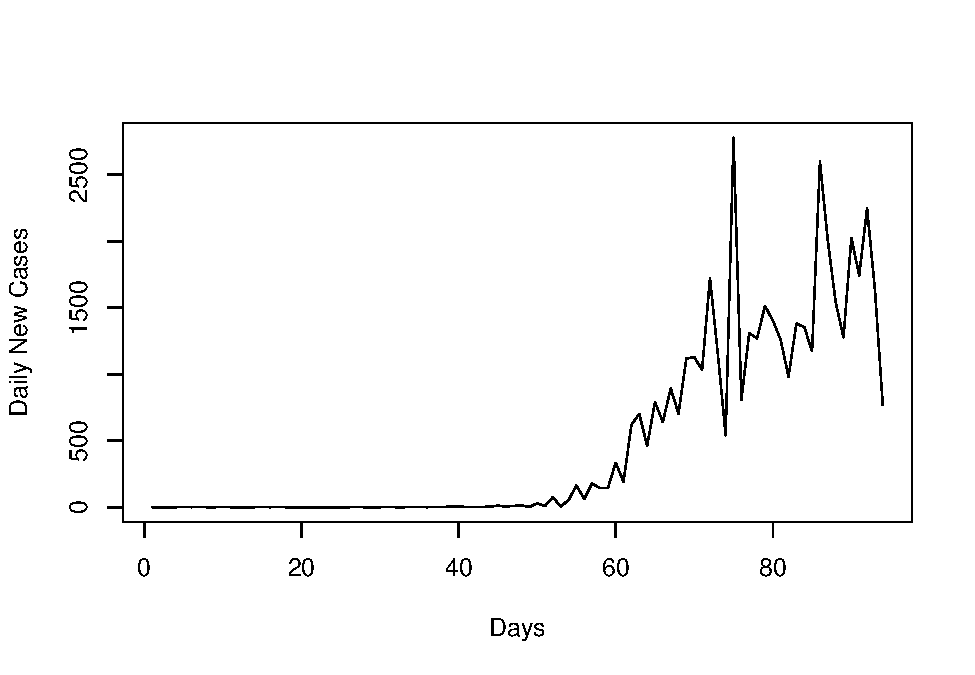
\includegraphics{Covid19Canada_files/figure-latex/unnamed-chunk-3-1.pdf}

\begin{Shaded}
\begin{Highlighting}[]
\KeywordTok{acf}\NormalTok{(}\KeywordTok{diff}\NormalTok{(canada}\OperatorTok{$}\NormalTok{new))}
\end{Highlighting}
\end{Shaded}

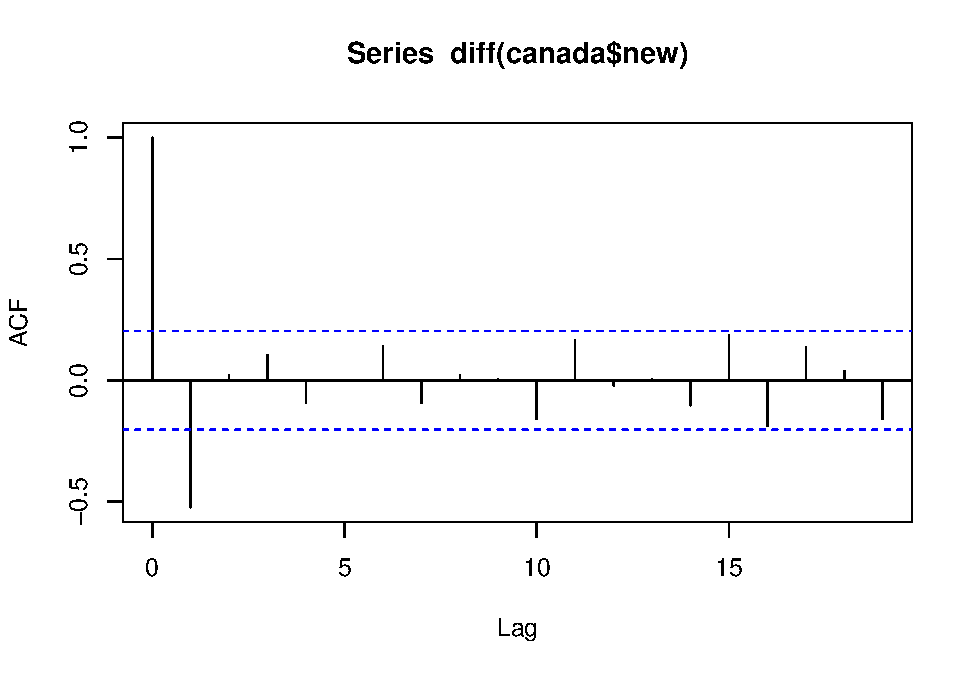
\includegraphics{Covid19Canada_files/figure-latex/unnamed-chunk-3-2.pdf}

\begin{Shaded}
\begin{Highlighting}[]
\KeywordTok{plot}\NormalTok{(}\KeywordTok{diff}\NormalTok{(canada}\OperatorTok{$}\NormalTok{new))}
\end{Highlighting}
\end{Shaded}

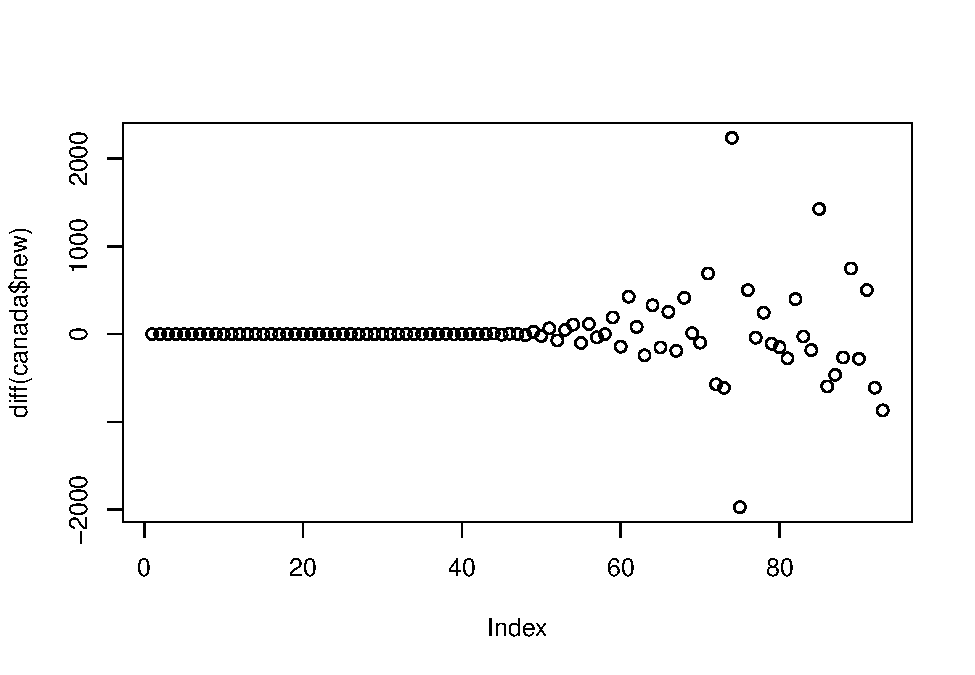
\includegraphics{Covid19Canada_files/figure-latex/unnamed-chunk-3-3.pdf}

\begin{Shaded}
\begin{Highlighting}[]
\NormalTok{arima\_cases \textless{}{-}}\StringTok{ }\KeywordTok{auto.arima}\NormalTok{(canada}\OperatorTok{$}\NormalTok{new, }\DataTypeTok{seasonal =}\NormalTok{ F)}
\NormalTok{arima\_cases}
\end{Highlighting}
\end{Shaded}

\begin{verbatim}
## Series: canada$new 
## ARIMA(0,1,3) with drift 
## 
## Coefficients:
##           ma1     ma2     ma3    drift
##       -0.9890  0.1911  0.3089  13.7211
## s.e.   0.1013  0.1418  0.1880  15.7687
## 
## sigma^2 estimated as 92460:  log likelihood=-662.54
## AIC=1335.08   AICc=1335.77   BIC=1347.75
\end{verbatim}

\begin{Shaded}
\begin{Highlighting}[]
\NormalTok{arima\_cases2 \textless{}{-}}\StringTok{ }\KeywordTok{arima}\NormalTok{(canada}\OperatorTok{$}\NormalTok{new, }\DataTypeTok{order=}\KeywordTok{c}\NormalTok{(}\DecValTok{2}\NormalTok{, }\DecValTok{1}\NormalTok{, }\DecValTok{3}\NormalTok{))}
\NormalTok{arima\_cases2}
\end{Highlighting}
\end{Shaded}

\begin{verbatim}
## 
## Call:
## arima(x = canada$new, order = c(2, 1, 3))
## 
## Coefficients:
##          ar1      ar2      ma1     ma2      ma3
##       1.1303  -0.5149  -2.1928  1.9829  -0.6283
## s.e.  0.1996   0.1004   0.2202  0.3378   0.2098
## 
## sigma^2 estimated as 78673:  log likelihood = -659.32,  aic = 1330.63
\end{verbatim}

\begin{Shaded}
\begin{Highlighting}[]
\NormalTok{prediction\_time \textless{}{-}}\StringTok{ }\DecValTok{30}
\NormalTok{preds \textless{}{-}}\StringTok{ }\KeywordTok{forecast}\NormalTok{(arima\_cases2, }\DataTypeTok{h=}\DecValTok{30}\NormalTok{)}

\NormalTok{dates\textless{}{-}}\KeywordTok{c}\NormalTok{(}\KeywordTok{as.Date}\NormalTok{(canada}\OperatorTok{$}\NormalTok{date),}\KeywordTok{as.Date}\NormalTok{(}\KeywordTok{seq}\NormalTok{(}\KeywordTok{as.Date}\NormalTok{(canada}\OperatorTok{$}\NormalTok{date[}\KeywordTok{nrow}\NormalTok{(canada)]),}\DataTypeTok{by=}\StringTok{"day"}\NormalTok{,}\DataTypeTok{length.out =}\NormalTok{ prediction\_time}\OperatorTok{+}\DecValTok{1}\NormalTok{)))}
\NormalTok{a \textless{}{-}}\KeywordTok{plot}\NormalTok{(preds,}\DataTypeTok{xaxt=}\StringTok{\textquotesingle{}n\textquotesingle{}}\NormalTok{,}\DataTypeTok{main=}\NormalTok{(}\StringTok{"Forecast of daily confirmed cases {-} Canada"}\NormalTok{), }\DataTypeTok{ylab=}\StringTok{"Number of New Cases"}\NormalTok{)}
\NormalTok{at  \textless{}{-}}\StringTok{  }\KeywordTok{seq}\NormalTok{(}\DecValTok{1}\NormalTok{,}\KeywordTok{nrow}\NormalTok{(canada)}\OperatorTok{+}\NormalTok{prediction\_time,}\DataTypeTok{length.out=}\DecValTok{12}\NormalTok{)}
\KeywordTok{axis}\NormalTok{(}\DecValTok{1}\NormalTok{, }\DataTypeTok{at =}\NormalTok{ at}\OperatorTok{+}\DecValTok{5}\NormalTok{, }\DataTypeTok{labels =}\NormalTok{ dates[at],}\DataTypeTok{cex.axis =} \FloatTok{.7}\NormalTok{,}\DataTypeTok{las=}\DecValTok{3}\NormalTok{) }
\end{Highlighting}
\end{Shaded}

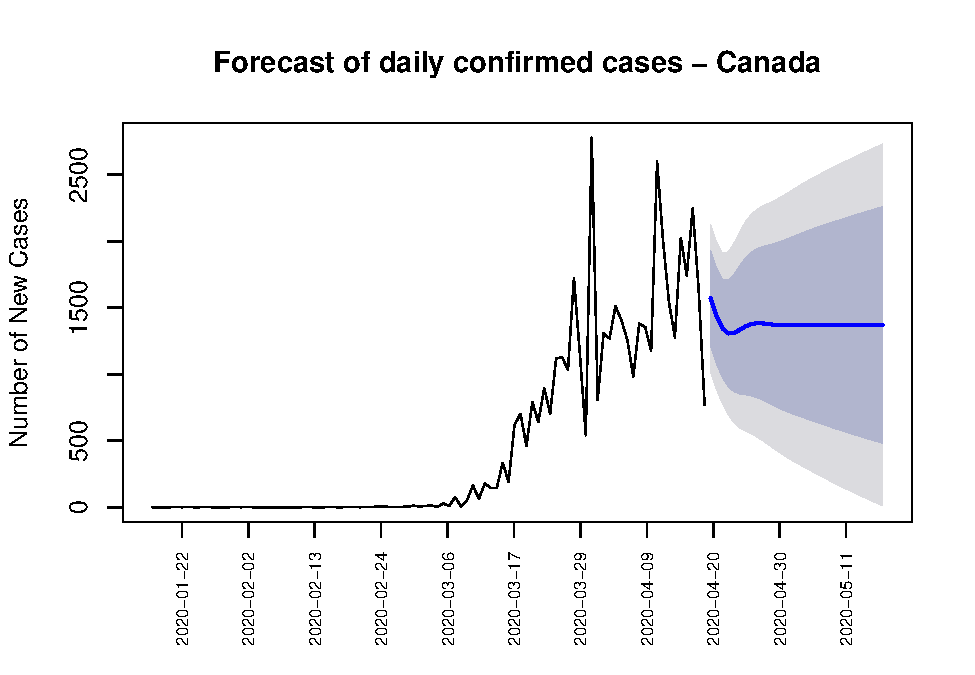
\includegraphics{Covid19Canada_files/figure-latex/unnamed-chunk-3-4.pdf}

\hypertarget{daily-cases-for-canada---normalized}{%
\subsection{Daily cases for Canada -
Normalized}\label{daily-cases-for-canada---normalized}}

\begin{Shaded}
\begin{Highlighting}[]
\NormalTok{tests \textless{}{-}}\StringTok{ }\KeywordTok{read.csv}\NormalTok{(}\StringTok{"/Users/Sofia/Desktop/Data583Project/canada{-}covid19/testing\_cumulative.csv"}\NormalTok{, }\DataTypeTok{stringsAsFactors =}\NormalTok{ F)}

\NormalTok{tests \textless{}{-}}\StringTok{ }\KeywordTok{select}\NormalTok{(tests, date\_testing, cumulative\_testing)}
\KeywordTok{setnames}\NormalTok{(tests, }\DataTypeTok{old =} \KeywordTok{c}\NormalTok{(}\StringTok{\textquotesingle{}date\_testing\textquotesingle{}}\NormalTok{, }\StringTok{\textquotesingle{}cumulative\_testing\textquotesingle{}}\NormalTok{), }\DataTypeTok{new =} \KeywordTok{c}\NormalTok{(}\StringTok{\textquotesingle{}Date\textquotesingle{}}\NormalTok{, }\StringTok{\textquotesingle{}csum\textquotesingle{}}\NormalTok{))}
\NormalTok{tests}\OperatorTok{$}\NormalTok{Date \textless{}{-}}\StringTok{ }\KeywordTok{as.Date}\NormalTok{(tests}\OperatorTok{$}\NormalTok{Date, }\StringTok{"\%d{-}\%m{-}\%Y"}\NormalTok{)}

\NormalTok{tests \textless{}{-}}\StringTok{ }\NormalTok{tests }\OperatorTok{\%\textgreater{}\%}\KeywordTok{group\_by}\NormalTok{(Date) }\OperatorTok{\%\textgreater{}\%}\StringTok{ }\KeywordTok{summarise}\NormalTok{(}\DataTypeTok{cumulative\_tests=} \KeywordTok{sum}\NormalTok{(csum))}

\NormalTok{new\_tests \textless{}{-}}\StringTok{ }\KeywordTok{diff}\NormalTok{(tests}\OperatorTok{$}\NormalTok{cumulative\_tests, }\DataTypeTok{differences =} \DecValTok{1}\NormalTok{)}

\NormalTok{new\_tests \textless{}{-}}\StringTok{ }\KeywordTok{c}\NormalTok{(}\DecValTok{0}\NormalTok{, new\_tests)}
\NormalTok{tests}\OperatorTok{$}\NormalTok{daily\_tests \textless{}{-}}\StringTok{ }\NormalTok{new\_tests}
\KeywordTok{setnames}\NormalTok{(tests, }\DataTypeTok{old =} \KeywordTok{c}\NormalTok{(}\StringTok{\textquotesingle{}Date\textquotesingle{}}\NormalTok{), }\DataTypeTok{new =} \KeywordTok{c}\NormalTok{(}\StringTok{\textquotesingle{}date\textquotesingle{}}\NormalTok{))}

\NormalTok{canada}
\end{Highlighting}
\end{Shaded}

\begin{verbatim}
## # A tibble: 94 x 3
##    date       total_cases   new
##    <date>           <int> <dbl>
##  1 2020-01-22           0     0
##  2 2020-01-23           0     0
##  3 2020-01-24           0     0
##  4 2020-01-25           0     0
##  5 2020-01-26           1     1
##  6 2020-01-27           1     0
##  7 2020-01-28           2     1
##  8 2020-01-29           2     0
##  9 2020-01-30           2     0
## 10 2020-01-31           4     2
## # ... with 84 more rows
\end{verbatim}

\begin{Shaded}
\begin{Highlighting}[]
\NormalTok{canada\_normal \textless{}{-}}\StringTok{ }\KeywordTok{inner\_join}\NormalTok{(canada, tests, }\DataTypeTok{by =} \StringTok{\textquotesingle{}date\textquotesingle{}}\NormalTok{)}

\NormalTok{canada\_normal}\OperatorTok{$}\NormalTok{proportion \textless{}{-}}\StringTok{ }\NormalTok{canada\_normal}\OperatorTok{$}\NormalTok{new}\OperatorTok{/}\NormalTok{canada\_normal}\OperatorTok{$}\NormalTok{daily\_tests}
\CommentTok{\#\#\#\#\#\#\#\#\#\#\#\#\#\#\#\#\#\#\#\#\#\#\#\#\#\#\#\#\#\#\#\#\#\#\#\#\#\#\#\#\#\#\#\#\#\#\#\#\#\#\#\#\#\#\#\#\#\#\#\#\#\#}

\NormalTok{ts\_cases\_normalized \textless{}{-}}\StringTok{ }\KeywordTok{ts}\NormalTok{(canada\_normal}\OperatorTok{$}\NormalTok{proportion)}
\KeywordTok{ts.plot}\NormalTok{(ts\_cases\_normalized, }\DataTypeTok{xlab=}\StringTok{"Days"}\NormalTok{, }\DataTypeTok{ylab=}\StringTok{"Positive daily cases (normalized)"}\NormalTok{)}
\end{Highlighting}
\end{Shaded}

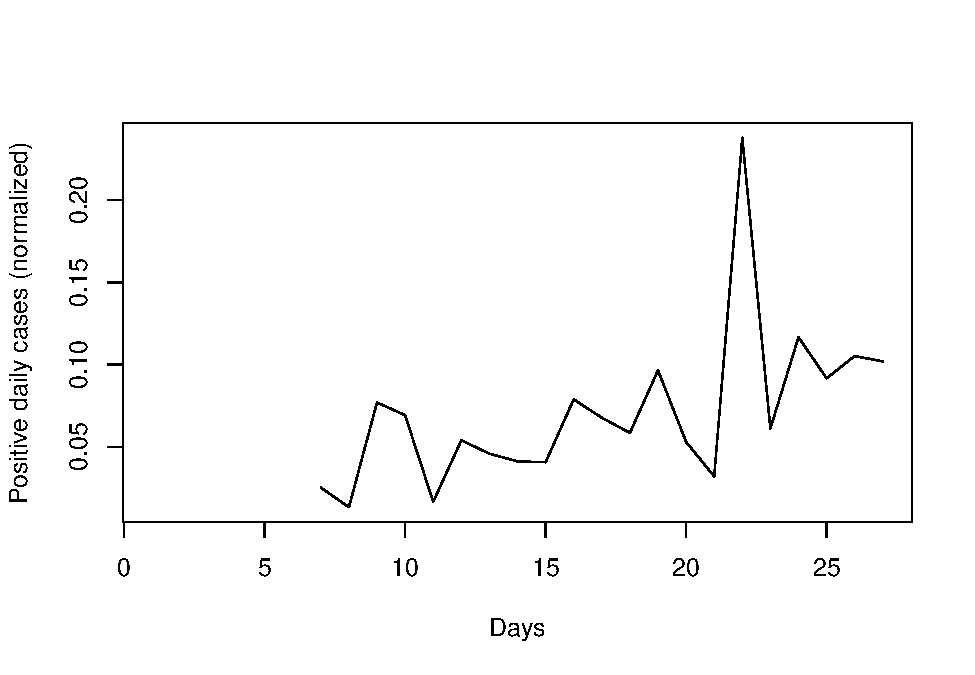
\includegraphics{Covid19Canada_files/figure-latex/unnamed-chunk-4-1.pdf}

\begin{Shaded}
\begin{Highlighting}[]
\NormalTok{canada\_normal \textless{}{-}}\StringTok{ }\KeywordTok{drop\_na}\NormalTok{(canada\_normal)}
\KeywordTok{acf}\NormalTok{(}\KeywordTok{diff}\NormalTok{(canada\_normal}\OperatorTok{$}\NormalTok{proportion, }\DecValTok{2}\NormalTok{))}
\end{Highlighting}
\end{Shaded}

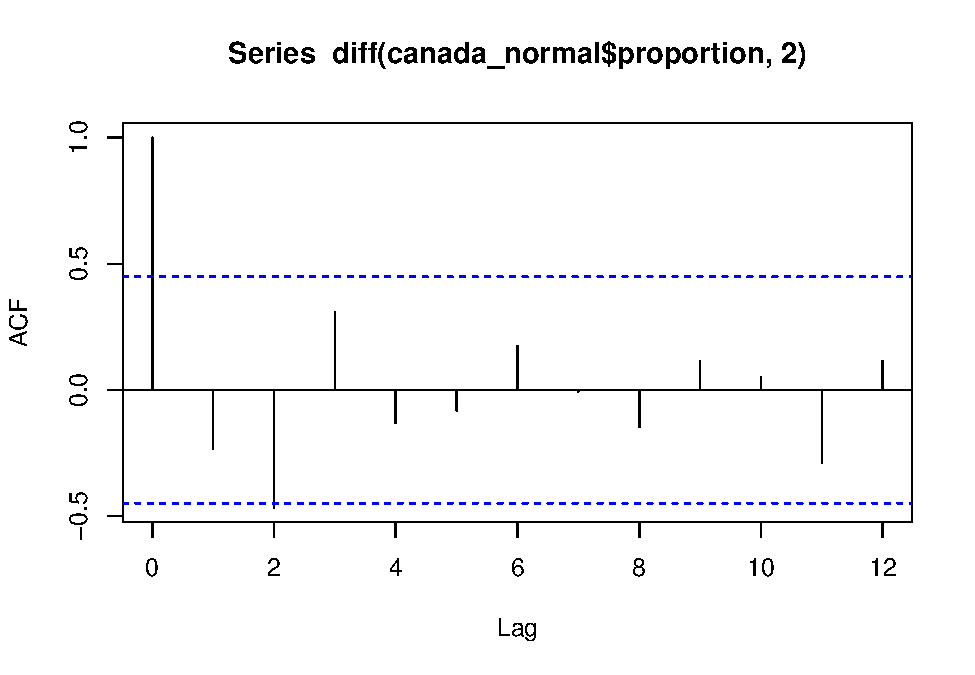
\includegraphics{Covid19Canada_files/figure-latex/unnamed-chunk-4-2.pdf}

\begin{Shaded}
\begin{Highlighting}[]
\NormalTok{arima\_cases\_normal \textless{}{-}}\StringTok{ }\KeywordTok{auto.arima}\NormalTok{(canada\_normal}\OperatorTok{$}\NormalTok{proportion, }\DataTypeTok{seasonal =}\NormalTok{ F)}
\NormalTok{arima\_cases\_normal}
\end{Highlighting}
\end{Shaded}

\begin{verbatim}
## Series: canada_normal$proportion 
## ARIMA(0,1,2) 
## 
## Coefficients:
##           ma1     ma2
##       -1.2007  0.4933
## s.e.   0.2669  0.2673
## 
## sigma^2 estimated as 0.002013:  log likelihood=33.96
## AIC=-61.91   AICc=-60.41   BIC=-58.92
\end{verbatim}

\begin{Shaded}
\begin{Highlighting}[]
\NormalTok{arima\_cases\_normal2 \textless{}{-}}\StringTok{ }\KeywordTok{arima}\NormalTok{(canada\_normal}\OperatorTok{$}\NormalTok{proportion, }\DataTypeTok{order=}\KeywordTok{c}\NormalTok{(}\DecValTok{7}\NormalTok{, }\DecValTok{2}\NormalTok{, }\DecValTok{2}\NormalTok{))}
\NormalTok{arima\_cases\_normal2}
\end{Highlighting}
\end{Shaded}

\begin{verbatim}
## 
## Call:
## arima(x = canada_normal$proportion, order = c(7, 2, 2))
## 
## Coefficients:
##           ar1      ar2      ar3      ar4      ar5     ar6     ar7      ma1
##       -0.6851  -0.4341  -0.2457  -0.1826  -0.0609  0.3061  0.2527  -1.5823
## s.e.   1.1252   1.4586   1.4268   1.2465   1.0845  0.9325  0.4452   1.1205
##          ma2
##       0.5823
## s.e.  1.0762
## 
## sigma^2 estimated as 0.001416:  log likelihood = 30.87,  aic = -41.74
\end{verbatim}

\begin{Shaded}
\begin{Highlighting}[]
\NormalTok{prediction\_time \textless{}{-}}\StringTok{ }\DecValTok{30}
\NormalTok{preds2 \textless{}{-}}\StringTok{ }\KeywordTok{forecast}\NormalTok{(arima\_cases\_normal2, }\DataTypeTok{h=}\DecValTok{30}\NormalTok{)}

\NormalTok{dates\textless{}{-}}\KeywordTok{c}\NormalTok{(}\KeywordTok{as.Date}\NormalTok{(canada\_normal}\OperatorTok{$}\NormalTok{date),}\KeywordTok{as.Date}\NormalTok{(}\KeywordTok{seq}\NormalTok{(}\KeywordTok{as.Date}\NormalTok{(canada\_normal}\OperatorTok{$}\NormalTok{date[}\KeywordTok{nrow}\NormalTok{(canada\_normal)]),}\DataTypeTok{by=}\StringTok{"day"}\NormalTok{,}\DataTypeTok{length.out =}\NormalTok{ prediction\_time}\OperatorTok{+}\DecValTok{1}\NormalTok{)))}
\KeywordTok{plot}\NormalTok{(preds2,}\DataTypeTok{xaxt=}\StringTok{\textquotesingle{}n\textquotesingle{}}\NormalTok{,}\DataTypeTok{main=}\NormalTok{(}\StringTok{"Forecast of Normalized Cases (proportion)"}\NormalTok{), }\DataTypeTok{ylab=}\StringTok{"Positive daily cases (normalized)"}\NormalTok{)}
\NormalTok{at  \textless{}{-}}\StringTok{  }\KeywordTok{seq}\NormalTok{(}\DecValTok{1}\NormalTok{,}\KeywordTok{nrow}\NormalTok{(canada\_normal)}\OperatorTok{+}\NormalTok{prediction\_time,}\DataTypeTok{length.out=}\DecValTok{12}\NormalTok{)}
\KeywordTok{axis}\NormalTok{(}\DecValTok{1}\NormalTok{, }\DataTypeTok{at =}\NormalTok{ at}\OperatorTok{+}\DecValTok{3}\NormalTok{, }\DataTypeTok{labels =}\NormalTok{ dates[at],}\DataTypeTok{cex.axis =} \FloatTok{.7}\NormalTok{,}\DataTypeTok{las=}\DecValTok{3}\NormalTok{)}
\end{Highlighting}
\end{Shaded}

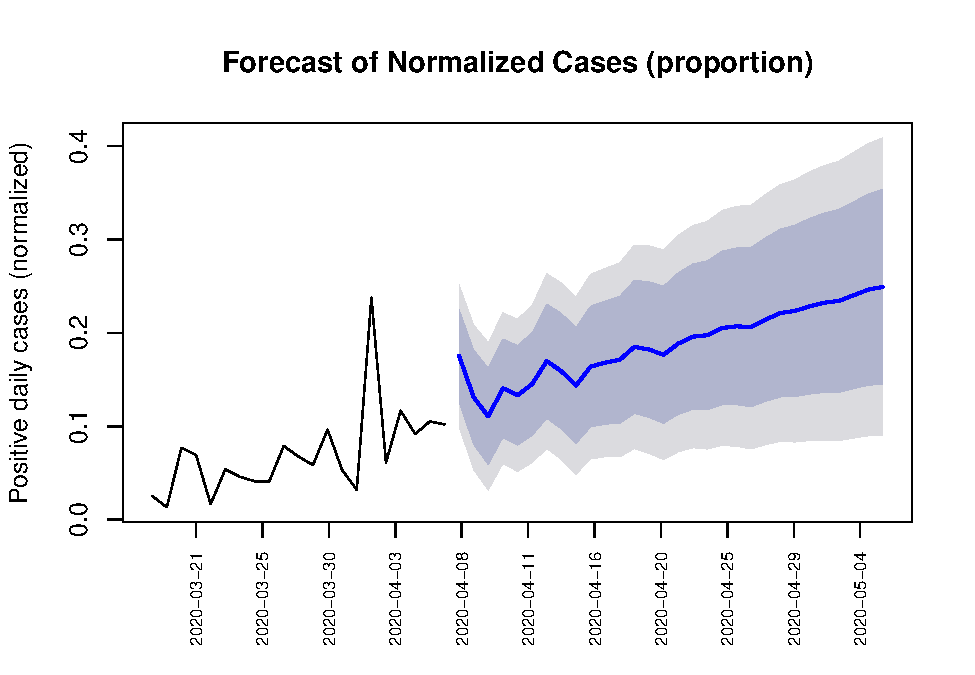
\includegraphics{Covid19Canada_files/figure-latex/unnamed-chunk-4-3.pdf}

\hypertarget{not-using-this-part}{%
\paragraph{Not using this part \ldots{}}\label{not-using-this-part}}

\hypertarget{canada-wide-cumulative}{%
\subsection{Canada-wide Cumulative}\label{canada-wide-cumulative}}

\begin{Shaded}
\begin{Highlighting}[]
\CommentTok{\#cumulative cases}
\NormalTok{cumulative \textless{}{-}}\StringTok{ }\KeywordTok{aggregate}\NormalTok{(data\_long}\OperatorTok{$}\NormalTok{n, }\DataTypeTok{by=}\KeywordTok{list}\NormalTok{(}\DataTypeTok{Category=}\NormalTok{data\_long}\OperatorTok{$}\NormalTok{date\_report), }\DataTypeTok{FUN=}\NormalTok{sum)}

\NormalTok{ts\_cases \textless{}{-}}\StringTok{ }\KeywordTok{ts}\NormalTok{(cumulative}\OperatorTok{$}\NormalTok{x)}
\KeywordTok{ts.plot}\NormalTok{(ts\_cases, }\DataTypeTok{xlab=}\StringTok{"Days"}\NormalTok{, }\DataTypeTok{ylab=}\StringTok{"Cumulative Cases"}\NormalTok{)}
\end{Highlighting}
\end{Shaded}

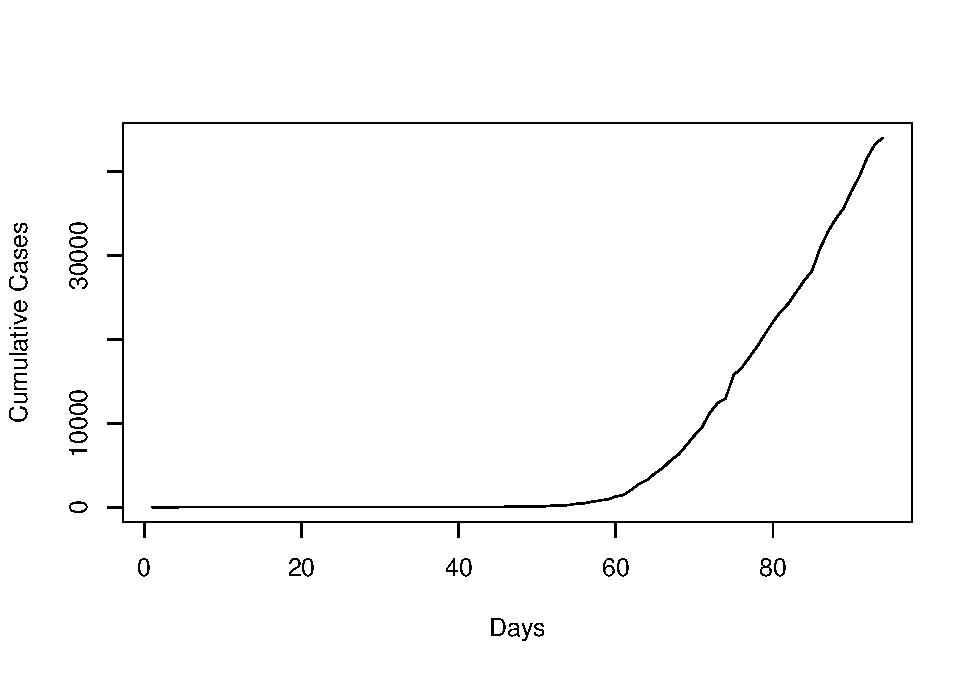
\includegraphics{Covid19Canada_files/figure-latex/unnamed-chunk-5-1.pdf}

\hypertarget{arima-for-cumulative-im-not-sure-if-this-is-usefuli-thought-arima-was-to-observe-patterns-in-the-daily-data-cumulative-data-shows-entirely-different-pattern.}{%
\subsection{ARIMA for cumulative (I'm not sure if this is useful\ldots I
thought ARIMA was to observe patterns in the daily data, cumulative data
shows entirely different pattern.
)}\label{arima-for-cumulative-im-not-sure-if-this-is-usefuli-thought-arima-was-to-observe-patterns-in-the-daily-data-cumulative-data-shows-entirely-different-pattern.}}

\begin{Shaded}
\begin{Highlighting}[]
\CommentTok{\#daily cases}
\NormalTok{arima\_cases\_cumulative \textless{}{-}}\StringTok{ }\KeywordTok{auto.arima}\NormalTok{(cumulative}\OperatorTok{$}\NormalTok{x, }\DataTypeTok{seasonal =}\NormalTok{ F)}
\NormalTok{arima\_cases\_cumulative}
\end{Highlighting}
\end{Shaded}

\begin{verbatim}
## Series: cumulative$x 
## ARIMA(2,2,1) 
## 
## Coefficients:
##           ar1      ar2      ma1
##       -0.4624  -0.2730  -0.4612
## s.e.   0.1635   0.1373   0.1390
## 
## sigma^2 estimated as 100307:  log likelihood=-659.26
## AIC=1326.52   AICc=1326.98   BIC=1336.61
\end{verbatim}

\begin{Shaded}
\begin{Highlighting}[]
\NormalTok{preds\_cumulative \textless{}{-}}\StringTok{ }\KeywordTok{forecast}\NormalTok{(arima\_cases\_cumulative, }\DataTypeTok{h=}\DecValTok{30}\NormalTok{)}
\KeywordTok{plot}\NormalTok{(preds\_cumulative)}
\end{Highlighting}
\end{Shaded}

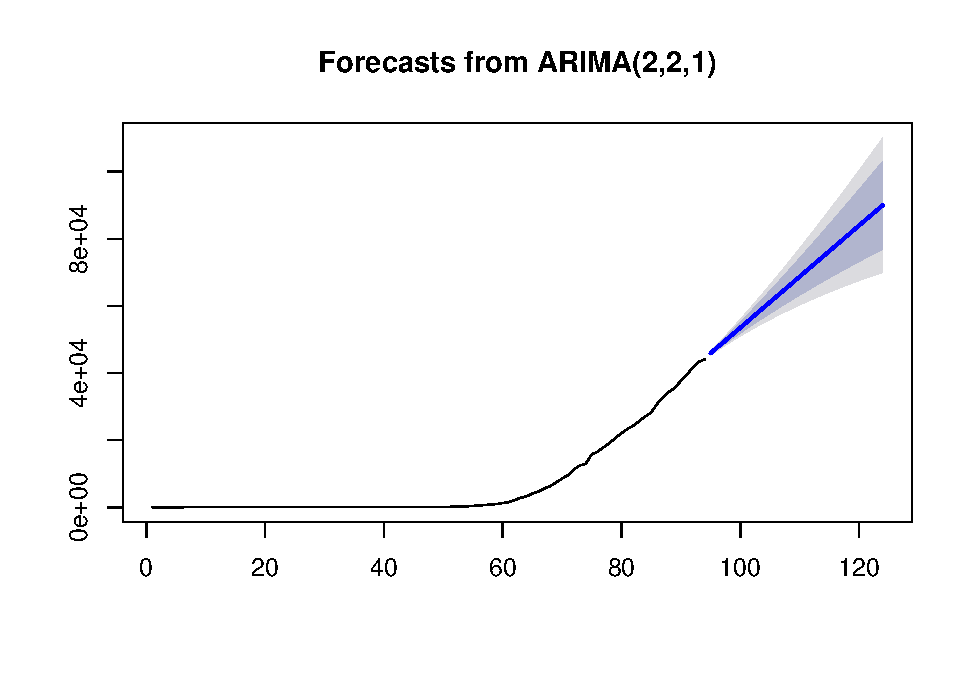
\includegraphics{Covid19Canada_files/figure-latex/unnamed-chunk-6-1.pdf}

\hypertarget{province-breakdown---cumulative}{%
\subsection{Province Breakdown -
Cumulative}\label{province-breakdown---cumulative}}

\begin{Shaded}
\begin{Highlighting}[]
\CommentTok{\# cases by province}
\NormalTok{cases\_prov \textless{}{-}}\StringTok{ }\KeywordTok{aggregate}\NormalTok{(data\_long}\OperatorTok{$}\NormalTok{n, }\DataTypeTok{by=}\KeywordTok{list}\NormalTok{(}\DataTypeTok{Category=}\NormalTok{data\_long}\OperatorTok{$}\NormalTok{date\_report, data\_long}\OperatorTok{$}\NormalTok{Province.State), }\DataTypeTok{FUN=}\NormalTok{sum)}
\NormalTok{DT \textless{}{-}}\StringTok{ }\KeywordTok{data.table}\NormalTok{(cases\_prov, }\DataTypeTok{key =} \StringTok{"Group.2"}\NormalTok{)}
\NormalTok{DT \textless{}{-}}\StringTok{ }\NormalTok{DT[, csum }\OperatorTok{:}\ErrorTok{=}\StringTok{ }\KeywordTok{cumsum}\NormalTok{(x), by =}\StringTok{ }\KeywordTok{key}\NormalTok{(DT)]}
\KeywordTok{setnames}\NormalTok{(DT, }\DataTypeTok{old =} \KeywordTok{c}\NormalTok{(}\StringTok{\textquotesingle{}Category\textquotesingle{}}\NormalTok{,}\StringTok{\textquotesingle{}Group.2\textquotesingle{}}\NormalTok{), }\DataTypeTok{new =} \KeywordTok{c}\NormalTok{(}\StringTok{\textquotesingle{}date\textquotesingle{}}\NormalTok{,}\StringTok{\textquotesingle{}province\textquotesingle{}}\NormalTok{))}

\KeywordTok{ggplot}\NormalTok{(}\DataTypeTok{data=}\NormalTok{DT,}
       \KeywordTok{aes}\NormalTok{(}\DataTypeTok{x=}\NormalTok{DT}\OperatorTok{$}\NormalTok{date, }\DataTypeTok{y=}\NormalTok{DT}\OperatorTok{$}\NormalTok{csum, }\DataTypeTok{colour=}\NormalTok{DT}\OperatorTok{$}\NormalTok{province)) }\OperatorTok{+}
\StringTok{       }\KeywordTok{geom\_line}\NormalTok{()}
\end{Highlighting}
\end{Shaded}

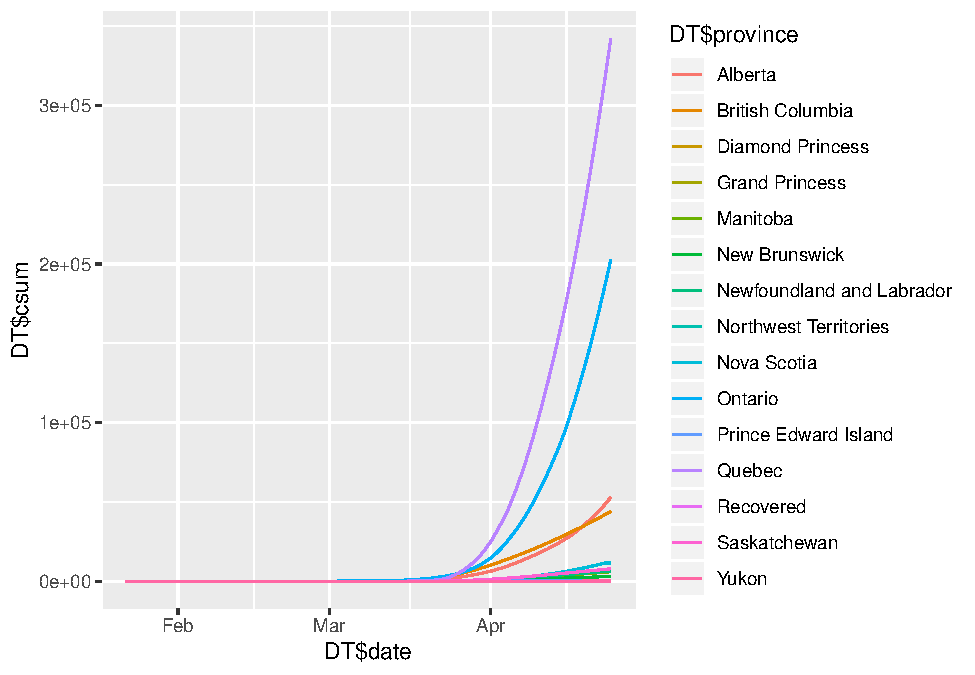
\includegraphics{Covid19Canada_files/figure-latex/unnamed-chunk-7-1.pdf}

\begin{Shaded}
\begin{Highlighting}[]
\NormalTok{DT\_reduced \textless{}{-}}\StringTok{ }\KeywordTok{subset}\NormalTok{(DT, DT}\OperatorTok{$}\NormalTok{province }\OperatorTok{==}\StringTok{ }\KeywordTok{c}\NormalTok{(}\StringTok{\textquotesingle{}Alberta\textquotesingle{}}\NormalTok{, }\StringTok{\textquotesingle{}British Columbia\textquotesingle{}}\NormalTok{, }\StringTok{\textquotesingle{}Ontario\textquotesingle{}}\NormalTok{, }\StringTok{\textquotesingle{}Quebec\textquotesingle{}}\NormalTok{))}
\end{Highlighting}
\end{Shaded}

\begin{verbatim}
## Warning in DT$province == c("Alberta", "British Columbia", "Ontario",
## "Quebec"): longer object length is not a multiple of shorter object length
\end{verbatim}

\begin{Shaded}
\begin{Highlighting}[]
\KeywordTok{ggplot}\NormalTok{(}\DataTypeTok{data=}\NormalTok{DT\_reduced,}
       \KeywordTok{aes}\NormalTok{(}\DataTypeTok{x=}\NormalTok{DT\_reduced}\OperatorTok{$}\NormalTok{date, }\DataTypeTok{y=}\NormalTok{DT\_reduced}\OperatorTok{$}\NormalTok{csum, }\DataTypeTok{colour=}\NormalTok{DT\_reduced}\OperatorTok{$}\NormalTok{province)) }\OperatorTok{+}
\StringTok{       }\KeywordTok{geom\_line}\NormalTok{()}
\end{Highlighting}
\end{Shaded}

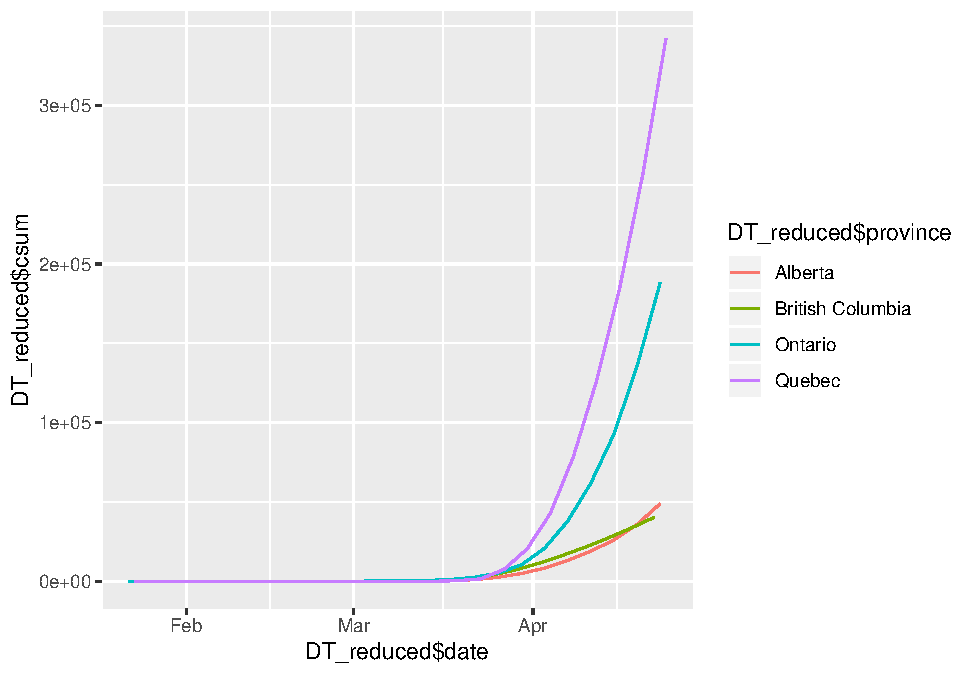
\includegraphics{Covid19Canada_files/figure-latex/unnamed-chunk-7-2.pdf}


\end{document}
